%
% Reproducibility manuscript: describe results from relative
% alchemical free energy simulation done with various MD packages.
%
% arara: make
% arara: pdflatex
% arara: bibtex
% arara: pdflatex
% arara: pdflatex
% arara: clean: {files: [reprod.aux, reprod.bbl, reprod.blg, reprod.log,
%acs-reprod.bib, reprod.lod, reprod.fls]}
%

\documentclass[journal=jctcce,manuscript=article]{achemso}

\usepackage[T1]{fontenc}
\usepackage{graphicx}
\usepackage{amsmath,amssymb,mathrsfs}
\usepackage{xr}
\usepackage{booktabs}
\usepackage{multirow}
\usepackage{rotating}
\usepackage{siunitx}
\usepackage{nameref}
\usepackage{easy-todo}

\usepackage{arydshln}


\usepackage{footref}


\externaldocument[S-]{SI}

\sisetup{
  separate-uncertainty = true
}

\newcommand{\progname}[1]{\texttt{#1}}
\newcommand{\inpopt}[1]{\texttt{#1}}

\renewcommand{\vec}[1]{\mathbf{#1}}
\renewcommand{\footnoterule}{}


\title{Are Alchemical Free Energy Calculations Reproducible?}

\author{Hannes H. Loeffler}
\affiliation[Scientific Computing Department, STFC]{Science \&
  Technology Facilities Council, Daresbury, Warrington WA4 4AD,
  United Kingdom}
\altaffiliation{Current address: Eli Lilly and Company,
  Erl Wood Manor, Sunninghill Road, Windlesham GU20 6PH,
  United Kingdom}
\email{Hannes.Loeffler@gmail.com}
\phone{+44 1276 483354}

\author{Stefano Bosisio}
\affiliation[University of Edinburgh]{EaStCHEM School of Chemistry,
  University of Edinburgh, David Brewster Road, Edinburgh EH9 3FJ, 
  United Kingdom}

\author{Guilherme Duarte Ramos Matos}
\affiliation[University of California, Irvine]{Department of
  Chemistry, University of California, Irvine}

\author{Donghyuk Suh}
\affiliation[University of Chicago]{University of Chicago}

\author{Benoit Roux}
\affiliation[University of Chicago]{University of Chicago}

\author{David L. Mobley}
\affiliation[University of California, Irvine]{Departments of
  Pharmaceutical Sciences and Chemistry, University of California,
  Irvine}

\author{Julien Michel}
\affiliation[University of Edinburgh]{EaStCHEM School of Chemistry,
  University of Edinburgh, David Brewster Road, Edinburgh EH9 3FJ,
  United Kingdom}


\keywords{Free Energy, Hydration, Alchemical, Reproducibility, Automation}



\begin{document}

\begin{abstract}
  Alchemical free energy calculations are an increasingly important modern 
  simulation technique.  Contemporary molecular dynamics (MD) software such as AMBER, CHARMM, GROMACS and SOMD include support for the method. Implementation details vary among those codes but users expect reliability and reproducibility, i.e.\ for a given potential function, comparable free energy must be obtained within statistical bounds regardless of the code used.  \emph{Relative} alchemical free energy (RAFE) simulation is increasingly used to support molecular design activities, yet the reproducibility of the methodology has been less well tested than its absolute counterpart. Here we present the results for RAFE calculations for hydration free energies of a set of small 
  organic molecules and show that free energies can be satisfactorily 
  reproduced with aforementioned codes. However, this requires attention to 
  detail and package-specific protocols. The benchmarks and protocols reported 
  here should be useful for the community to validate new and future versions of free energy calculations software.
\end{abstract}

\begin{tocentry}
  % \includegraphics[scale=1.0]{}
\end{tocentry}


\section{Introduction}
\label{sec:intro}

The free energy is a fundamental function of thermodynamics as it explains 
how processes in nature evolve.  The equilibrium balance of products and reactants in a hypothetical chemical reaction can be immediately determined
from the knowledge of the free energy difference of reactants and
products and their concentrations.  The free energy landscape of a given 
system, however, can be very complicated and rugged with barriers which impose
limits on how fast the process can take place.  It is therefore of
little surprise that the determination of free energy changes is of
utmost importance in the natural sciences, e.g.\ for binding and
molecular association, solvation and solubility, protein folding and
stability, partition and transfer, and design and improvement of force
fields. 

The calculation of free energies via molecular 
simulations~\cite{hansen_practical_2014, doi:10.1021/jp102971x,
  Gallicchio201127, doi:10.1080/08927022.2015.1132317,
  doi:10.1146/annurev.matsci.32.111901.153708} has been particularly
attractive as it promises to circumvent certain limitations of experimental
approaches. Specifically, processes can be understood at the atomic level and there is the potential that computational techniques can be 
more cost and time effective, especially if they can predict the properties of new molecules before their synthesis.  
Thus, a multitude of methods have been devised
 to make reversible work estimates accessible through 
computation~\cite{hansen_practical_2014,
  doi:10.1021/jp102971x, Gallicchio201127,
  doi:10.1080/08927022.2015.1132317,
  doi:10.1146/annurev.matsci.32.111901.153708}.  However, the
reliability of estimates is still very much a matter of
concern~\cite{doi:10.1021/jp102971x, doi:10.1021/acs.jctc.5b00179}.

Here we are interested in \emph{alchemical} free energy methods because they 
are firmly rooted in statistical thermodynamics and thus give asymptotically 
correct free energy estimates, i.e.\ they are correct for a given potential 
energy function in the limit of sufficient simulation 
time~\cite{Beveridge-citeulike:3789890, straatsma:92, doi:10.1021/cr00023a004, 
hansen_practical_2014}.  The method has been applied in various forms for 
several decades now since the early days of computer 
simulation~\cite{doi:10.1063/1.1671118, bennett_efficient_1976, 
doi:10.1063/1.432264, FS9821700055,  Tembe1984281, doi:10.1063/1.449208}.  The 
method has gained renewed attention in recent years --- concomitant with 
improvements in computer hardware design --- within the traditional equilibrium
framework~\cite{GILSON19971047, doi:10.1021/jp0217839, deng_computations_2009} 
and also increasingly in combination with non-equilibrium 
techniques~\cite{ytreberg_comparison_2006, JCC:JCC23804,
  doi:10.1021/ct500964e}.  The name ``alchemical'' comes from the nonphysical
intermediates that often need to be created to obtain reliable estimates of 
free energy differences between physical end states, and because parts or 
all of a molecule may appear or disappear in a transformation.  In the 
context of force field methods the transformation takes place in parameter 
space, i.e.\ the various force field parameters are varied by scaling.  This 
can be a particularly efficient approach as it does not require sampling of 
diffusive motions, avoid crossing prohibitively large energy barriers if 
pathways are not well chosen and is easier to automate.

Alchemical free energy simulations rely on the concept of thermodynamic 
cycles~\cite{Tembe1984281}.
As the free energy is a state function, the sum of free energy changes
computed around any closed cycle must be zero.  This also implies
that the reversible work can be computed along
conveniently chosen legs of the cycle, even if the cycle is artificial.  For example, in
Fig.~\ref{fig:thermocycle} the relative free energy of hydration can
be computed along the vertical legs, that is, following the physical
process of moving a molecule from the gas phase to the liquid phase,
or along the horizontal legs in a non-physical but computationally more
efficient alchemical calculation.

\begin{figure}[ht]
  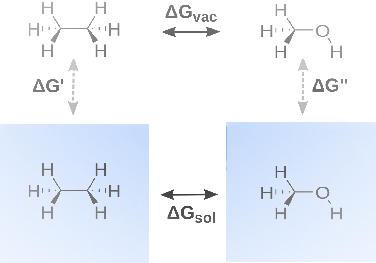
\includegraphics[scale=1.0]{figures/thermocycle.pdf}
  \caption{The thermodynamic cycle to compute the relative free energy
    of hydration
    $\Delta\Delta G_{\mathrm{hydr}}=\Delta G_{\mathrm{sol}}-\Delta
    G_{\mathrm{vac}}=\Delta G'' - \Delta G'$.  The example is for the
    ethanol $\leftrightarrow$ methanol transformation.  Alchemical
    simulations are performed along the non-physical horizontal
    legs while vertical legs illustrate the physical process of moving a 
    molecule from the vacuum to the solution.  The latter is also accessible 
    through absolute alchemical free energy simulation, see e.g.\ 
    Ref.~\citenum{doi:10.1021/acs.jced.7b00104}.}
  \label{fig:thermocycle}
\end{figure}
%DLM: What about making this look slightly more like a molecule? Particularly, I'm worried about the central proton in the methyl, which just comes out in a straight line from the O-C or C-C bond; it should go back from the plane or out from the plane. Can we use a "back from the plane" or "out from the plane" style bond like in organic chem?

Absolute (standard) alchemical free energy calculation has been of 
particular interest for many years~\cite{GILSON19971047,
  doi:10.1021/jp0217839, deng_computations_2009, ytreberg_comparison_2006, doi:10.1021/ct500964e, jorgensen1988efficient}.  \emph{Absolute}
here really means that the equilibrium constant of a physical
reaction, e.g.\ binding and dissociation, can be calculated directly
by completely decoupling or annihilating a whole molecule from its environment 
and the term is mostly being used to discriminate against techniques usually 
referred to as \emph{relative} (see below).  It should be emphasized that the 
``absolute'' approach still results in a \emph{relative} free energy,  
between the state where the solute fully interacts with its environment and the state where it does 
not.  Decoupling typically means the scaling of the non--bonded 
\emph{inter}--molecular interactions between the perturbed group (all atoms 
that differ in at least one force field parameter between the end states) and 
its environment.  We distinguish decoupling from annihilation, as the latter often includes a scaling of
the \emph{intra}--molecular interactions in addition to the 
inter--molecular interactions. 
% BR: This protocol turns a set of atoms into an ideal gas (no LJ, no bonds...). Is there any one who is rigorously this kind of annihilation? 
% I thought maybe only Bill Jorgensen in the early days was doing this with Monte Carlo... It literally cannot be done with MD.
These schemes may require two 
simulations along the opposite edges of a quadrilateral thermodynamic cycle 
but approaches that produce the reversible work directly in one simulation
have been proposed too~\cite{doi:10.1063/1.3519057, C3FD00125C}.

Relative alchemical free energy (RAFE) calculations mutate one molecule into 
another.  RAFEs have proven useful for instance to rank sets of related 
molecules according to their binding affinity for a given receptor.  This 
approach has recently gained increased traction in the context of relative free 
binding energies between small molecules, e.g.\ drug or lead like molecules and 
biomolecules~\cite{doi:10.1021/ja512751q, doi:10.1021/acs.jctc.6b00991}.

RAFEs can be calculated by making use of either the so-called single or dual topology method.

% BR: We should introduce dual topology before single topology, as it is conceptually simpler.
Dual topology means that \emph{all} 
atoms of the end states are duplicated and thus both sets are present at all
times but do not interact with each other \cite{doi:10.1021/j100056a020, doi:10.1021/jp981628n}.  Only non--bonded
interactions need to be scaled such that the disappearing end state
corresponds to an ideal gas molecule~\cite{doi:10.1021/jp981628n}.
The dual topology method is the most straightforward approach to compute RAFEs when the two molecules are structurally dissimilar.
Technically, a dual topology calculation is the same as two absolute calculations, executed simultaneously in opposite directions.  
This, however, comes with additional complications as the two independent
molecules can drift apart and sample completely different environments (e.g., binding site versus bulk solution).
%BR: This has some similarity with the wandering ligand problem, but adding too much here may lead to confusion.
%so suffer from the ``wandering'' ligand problem, as in absolute transformations\cite{Hermans-1986,Roux-bR-1996,GILSON19971047,Hermans-1997, doi:10.1021/jp0217839, deng_computations_2009}.  
It has been shown though that with the introduction of 
special restraints or constraints this can be a viable 
option~\cite{doi:10.1021/ct700081t,  rocklin_separated_2013, JCC:Axelsen-Li}.  
%BR: Actually, this procedure can be incorrect if the intramolecular terms are retained between the dummies. Then, there is double counting of those terms.
Restraints between corresponding atoms, thus emulating the single topology 
approach, can also be used without affecting the free 
energy~\cite{JCC:Axelsen-Li}.  A recent 
alternative~\cite{doi:10.1021/acs.jctc.5b00179} considered molecules with a
common core where all atom types are the same.  The charges that would be 
typically different in individual parameterization due to the local chemistry
were made equal.  This means that the core does not need to be duplicated and 
thus is not included in the mutation.  But all the chemistry is now exclusively 
handled by, possibly, just a few non--core atoms such that this approach may 
only be of limited use.

 
Single topology means that there is only one connected representation of the molecule to be transformed into another molecule.
% deleted: also implying a  single set of coordinates. 
% BR This is not true: in dual topology too there is a single set of coordinates 
Atoms of a given type are directly transformed, typically by linearly scaling the force field parameters, into atoms of a different type. 
The single topology method \cite{doi:10.1021/j100056a020, Michel2010,doi:10.1063/1.449208,doi:10.1021/j100056a020, doi:10.1021/jp981628n}
offers a straightforward route to implement RAFEs calculations~\cite{doi:10.1021/j100056a020, Michel2010}.
In typical implementations, 
a certain number of non-interacting ``dummy'' atoms must hold the place of disappearing/appearing atoms in order to balance the number of atoms in both end states.  
Dummy atoms have no non--bonded interactions in the end state but normally retain the bonded 
terms of the original atom to avoid complications with unbound 
atoms~\cite{doi:10.1021/jp981628n}.  
However, it is important to stress that a dummy atom should retain at most only
one angle term (Atom1-Atom2-Dummy) and one dihedral term (Atom1-Atom2-Atom3-Dummy) with respect to real atoms 
to yield correct results \cite{doi:10.1021/jp981628n,doi:10.1021/jp994193s}.
%
% BR: I cannot make sense of the rest of the paragraph. Also, you seem to ascribe this method only to AMBER and yet one reference is from me (with CHARMM). 
However this need not be. For instance, the AMBER 
implementation is a special case as it does not require the user to define 
dummy atoms explicitly, i.e.\ as atoms with coordinates and zero end state 
parameters in the topology, but only to mark the disappearing and appearing 
atoms in the control file of the MD engine.  
The contributions of bonded terms 
that involve at least one dummy atom will not be factored into the free energy 
as it is assumed that those contributions will perfectly cancel out in the 
thermodynamic cycle~\cite{doi:10.1021/acs.jcim.5b00057, doi:10.1021/jp994193s}.
%
The single topology approach~\cite{doi:10.1021/j100056a020} seeks to exploit the
topological and structural similarity of the two end states.
Chemical similarity is also of 
importance; e.g.\ chirality and binding modes where the relative three 
dimensional arrangement of groups in space must be taken into account.  
These considerations notwithstanding, the single topology approach is broadly applicable to a wide range of transformations.
For example, ring breaking is technically 
challenging~\cite{doi:10.1021/acs.jctc.6b00991} but it has also been
shown that this can be done in certain 
circumstances~\cite{doi:10.1021/acs.jcim.5b00057,
  doi:10.1021/jp994193s}.
Generally, modern MD software, e.g.\ AMBER~\cite{case_amber_2005},
CHARMM~\cite{JCC:JCC21287}, GROMACS~\cite{Abraham201519},
GROMOS~\cite{doi:10.1021/jp984217f} and SOMD~\cite{Sire-2016,
  doi:10.1021/ct300857j}, support a hybrid approach that combines aspects of single and dual topology~\cite{doi:10.1021/jp994193s}.


As alluded to above, consistency and reliability are the principal matter of concern.  
In particular, we need to ensure reproducibility of free energy results
among computer codes.  To the best of our knowledge this has not been
systematically tested yet for a set of different MD packages. 
However, there have been some recent efforts to test \emph{energy} 
reproducibility across packages~\cite{Shirts2017} --- a necessary but not 
sufficient prerequisite.  Another study went further and also compared liquid
densities across packages, revealing a variety of 
issues~\cite{doi:10.1021/acs.jctc.7b00489}.
For free energies, given a predefined force field and run--time parameters we 
ought to be able to obtain comparable free energy results within statistical 
convergence limits. This comparison has not yet been carried out.

In practice, one challenge to carry out such a comparison is that the methodologies
used in one MD program are not always available in another
package, or the same functionality is provided via different algorithms (e.g. algorithms for pressure and temperature 
scaling, integrators, etc).  Nevertheless, it is critical that free energy 
changes computed with different simulation software should be reproducible 
within statistical error, as this otherwise limits the transferability of 
potential energy functions, and the relevance of properties computed from a 
molecular simulation with a given package.  This is especially important as the community  
increasingly combines or swaps different simulation packages within workflows 
aimed at addressing challenging scientific 
problems~\cite{Pronk:2011:CNP:2063384.2063465, doi:10.1021/ci8000937, 
doi:10.1021/jp505332p, loeffler_fesetup:_2015, 
DBLP:journals/corr/Balasubramanian16g}.

In this work we present the results of relative hydration free energies of a 
set of small organic molecules (see Fig.~\ref{fig:cycles}).  Solvation free 
energies have a wide range of uses and various methods exist to compute
them~\cite{Skyner:2015:PCCP}.  They are also needed for calculations of a 
variety of important physical properties, and to calculate binding free 
energies where the simulation in solution (see Fig.~\ref{fig:thermocycle}) is 
combined with a mutation of the molecule bound to a 
partner~\cite{Skyner:2015:PCCP}.  A large database of hydration free energies 
computed from alchemical free energy (AFE) simulations, FreeSolv, has been 
presented recently~\cite{Mobley2014} and was just 
updated~\cite{doi:10.1021/acs.jced.7b00104}. Here, we focus on the 
reproducibility of RAFE with the simulation programs AMBER, CHARMM, GROMACS and 
SOMD.  We will discuss the reversible work results obtained with these packages 
and make recommendations regarding simulation protocols, setup procedures and 
analysis techniques.  We will also deliberate on what needs to be done to 
progress the field, both from a usability perspective as well as from the view 
point of code development.


\section{Methods}
\label{sec:methods}

We will compare relative free energies calculated via simultaneous parameter 
change simulations --- our ``unified protocol'' --- and separated parameter 
change simulations --- our ``split protocol''--- to relative free energy 
calculations obtained from two absolute hydration free energies -- our 
``absolute protocol''.  The unified protocol changes partial charges, van der Waals parameters, and bond parameters simultaneously along the alchemical path so that charge interactions and van der Waals interactions are varying simultaneously, while the split protocol separates the transformation of the van der Waals parameters from the charge transformation so that electrostatic interactions are modified separately from van der Waals interactions.
The order in which this has to be done is detailed in 
section~\ref{S-sec:separated}x of the SI.  In the split protocol, the scaling 
of the bonded terms can be combined with either transformation.


\subsection{Alchemical Free Energy Implementations}
\label{sec:afe_impl}

We begin by examining the differences in the alchemical free energy
implementations of the four MD codes we consider --- AMBER, CHARMM, GROMACS and
SOMD.  One key difference is in the softcore
functions~\cite{beutler_avoiding_1994, zacharias_separationshifted_1994} 
implemented in each code as summarized in section~\ref{S-sec:softcores}x of the 
SI.  Softcore functions are used to avoid the numerical 
stability problems of the conventional Lennard-Jones (LJ) and Coulombic inverse power law 
potentials~\cite{ISI:A1993MB07100015,steinbrecher_nonlinear_2007}, as they display singularities at 
zero distance (vertical asymptotes).  Attempting to modify interactions by 
linearly scaling back the LJ potential as a function of an 
interaction parameter, $\lambda$, causes the $r^{-12}$ to increasingly behave 
as a sharp repulsive singularity as $\lambda\rightarrow 0$ \cite{ISI:A1993MB07100015}.  This means that there 
is an unbounded discontinuous change between $\lambda = 0$ where particles can overlap, 
and $\lambda = \delta$, even as $\delta \rightarrow 0$, where particles still 
behave like minuscule hard spheres. This can lead to strongly 
fluctuating forces/energies and to severe instabilities in the integrator, as 
well as numerical errors in post processing analyses even when simulations do 
terminate normally~\cite{beutler_avoiding_1994, 
zacharias_separationshifted_1994, steinbrecher_nonlinear_2007}.

Another difference is how the codes scale force field parameters (``parameter 
scaling'') and/or the energy (``energy 
scaling'')~\cite{doi:10.1021/jp981628n}.  In the former case each parameter is 
scaled individually, e.g.\ in the case of a harmonic bond or angle term,
the force constant and the equilibrium distance/angle are scaled. In the 
latter case, the total energy is scaled, all at once or, equivalently for each 
individual force field contribution.  While free energy is a state function that
depends only on the end points, the mathematical pathways taken by the two methods through state space 
or alchemical space are different.  
% BR: Need to state this?
%It should be noted, however, that modification of Lennard-Jones 
%interactions is handled through softcore functions in modern codes (as is, in 
%some cases, that for electrostatic interactions) and thus parameter 
%scaling~\cite{doi:10.1021/j100056a020, JCROSS1986198} is now only used for 
%bonded terms and sometimes electrostatic interactions, at least in modern codes.

One more important issue is whether the code allows holonomic constraints to be applied 
to bonds, which change bond lengths in a transformation e.g.\ C--H to C--C.  
Changes in bond length need to account for the associated change in the free 
energy.  These and other details will be outlined below.

\paragraph{AMBER.}
This code is strictly dual topology and all terms are energy scaled.  The code 
allows, however, mapping of atoms in a single topology fashion and computes 
these non--softcore atoms  by linearly scaling the energy and forces for each 
atom in the pair.  The perturbed group must be entirely duplicated, i.e.\ for 
\progname{sander} this means two topology files with one end state each, and 
for \progname{pmemd} both end states in one topology file.  The softcore 
potential applies to any atom chosen by the user which may include atoms that 
actually have an equivalent in the other state.  Non--softcore atoms must still 
match 1:1 in both states.  
% BR: I do not understand what this means. It sounds very odd. 
Explicit dummy atoms are not needed as the code will 
only compute bonded contributions for ``real'' atoms and thus ignores bonded 
energies involving dummy atoms.  We will call this the ``implicit dummy 
protocol''. 
%
The code cannot handle bond length changes involving a constraint.  
There is only one global $\lambda$ for parameter transformation.  Protocols 
that couple only some parameters (split protocols, see below) must be emulated 
through careful construction of topologies e.g. by keeping fixed the LJ and bonded terms at the initial state for a charge transformation.  The setup for 
the two states must therefore use identical atom types for both end states 
while the charges are individually assigned.

% BR: Personally, I would not call PERT a dual topology. In fact, it is neither completely dual nor single. It depends on the user.
\paragraph{CHARMM.} The PERT module duplicates the topology similar to
\progname{sander} but mapped atoms are given in the topology only once.
The module requires balancing with explicit dummy atoms.  All energy terms are
linearly scaled by the coupling parameter $\lambda$.  The PSSP softcore potential is applied to \emph{all}
atoms in the perturbed group (see section~\ref{S-sec:softcores}x in the SI).  
The code can handle constraints of changing bond lengths in the perturbed group but this may cause incorrect results with PSSP softcores (Stefan Boresch, private communication).  There is only one global $\lambda$ for parameter
transformation, however, the scripting facilities in CHARMM allow run time
modification of topologies e.g.\ by setting charges or LJ parameters
to arbitrary values.

\paragraph{GROMACS.} This code uses a single topology description.
Bonded terms are strictly parameter--scaled, which requires proper
balancing of multi--term dihedrals i.e.\ each individual term in the Fourier 
series must have an equivalent in both end states.  If the term does not exist 
it must be created with parameters zeroing its energy.
The softcore potential applies to dummy 
atoms only determined from atoms having zero LJ parameters in the end states.
The code allows changing bond lengths involving constraints within the perturbed group  but this can lead to instabilities and wrong results (Michael Shirts, private communication).  There are separate $\lambda$s for LJ,
Coulomb and bonded parameters (and some other) which allows easy implementation 
of split protocols.

\paragraph{SOMD.} SOMD is a software built by linking  Sire~\cite{Sire-2016}
and OpenMM~\cite{doi:10.1021/ct300857j} molecular simulation libraries. 
This code uses a single topology description.
The final state is constructed at run time from the initial state with
a ``patch'' (list of force field parameters to be modified). All dummy atoms
needed to describe the transformation must be present in the initial state. 
Bond and angle terms are parameter--scaled while the dihedral term is
energy--scaled.  The softcore potential applies to atoms that become dummy atoms
 in one end-state. Dummy atoms are specified by a keyword in the patch file.
The code cannot handle constraints of changing bond lengths in the
perturbed group.  There is only one global $\lambda$ for parameter
scaling.  Separated protocols (see below) must be emulated through
careful construction of the patch file. 


\subsection{RAFE Setup}
\label{sec:rafe_setup}

The setup for all relative free energy simulations has been carried
out with the tool FESetup~\cite{loeffler_fesetup:_2015} (version
1.2).  FESetup is a perturbed topology writer for AMBER, CHARMM,
GROMACS, SOMD and also NAMD~\cite{JCC:JCC20289} (within the
limits of the dual topology approach).  The tool makes use of a
maximum common substructure search algorithm to automatically compute
atoms that can be mapped, i.e.\ atoms that have a direct relationship
to an equivalent atom in the other state -- atoms undergoing atom type conversion or modification.  The only current limit is that rings are
required to be preserved~\cite{doi:10.1021/acs.jcim.5b00057}.  With this
strategy a maximal single topology description is achieved: any atom that
does not match is made a dummy atom.  FESetup allows
equilibration of the solvated simulation systems and ensures that
``forward'' and ``backward'' simulations have the same number of
total atoms.  With SOMD the mass of each perturbed atom is taken as the mass of the heavier end-state atom (e.g. a hydrogen atom that is perturbed to a carbon atom has an atomic mass of 12 amu at all lambda values)  The masses of perturbed atoms are set to the mass of the heavier atom description  they are being perturbed to for SOMD.  The other codes use the atom masses of the initial state (AMBER, CHARMM) or allow the user to define how masses vary as a function of lambda (GROMACS).
% HHL: Donghyuk, please clarify!
The tool creates all input files with control
parameters, topologies and coordinates as required for RAFE
simulations.  Full details on FESetup can be found in
Ref.~\citenum{loeffler_fesetup:_2015}.

Figure~\ref{fig:cycles} shows all 18 transformation considered in the present study.
In the limit of sufficient sampling, RAFE simulations should not depend on the ``forward'' and ``backward'' direction of change with respect to the coupling 
parameter $\lambda$. But to test for possible discrepancies, we have run 
simulations in both directions.  As we shall discuss in the 
\nameref{sec:results} section we do see differences in some cases.

\begin{figure}[ht]
  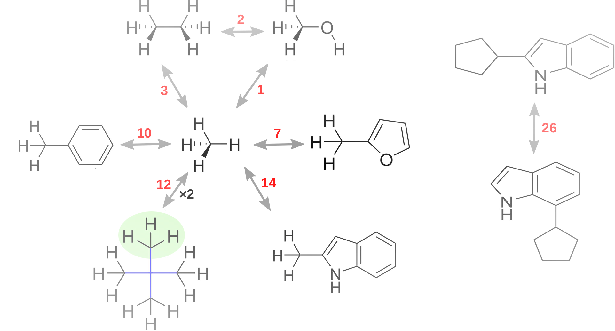
\includegraphics[scale=1.0]{figures/cycles.pdf}
  \caption{The thermodynamic cycles considered in this study.  To
    compute the free energy of hydration, all pair--wise
    transformations have to be carried out once in solution and once
    in vacuum.  Green and blue colours in neopentane show two
    alternative mappings for methane.  The numbers in red denote the
    number of dummy atoms.}
  \label{fig:cycles}
\end{figure}
%DLM: I have the same problem as noted above with the methyls in this figure; it'd be really nice to make them look a little more chemical. To some extent also true for neopentane's central carbon I think.

The ethane $\rightarrow$ methanol transformation is traditionally
regarded as a standard test for RAFE
simulations~\cite{doi:10.1063/1.449208, doi:10.1021/jp981629f}.   The
other transformations are centered around mutations from and to
methane, and are meant to mimic components of typical transformations that could be attempted
in the context of e.g.\ protein-ligand binding calculations. The 
2--cyclopentanylindole to 7--cyclopentanylindole (2--CPI to 7--CPI in our notation)
transformation has been added to include both deletion as well as
insertion of sub--parts of the perturbed group in one transformation, an aspect not tested by the other transformations.  For
neopentane $\rightarrow$ methane we point out that there are two
alternative mappings possible, see Figure~\ref{fig:cycles}.  One mapping has methane matched to a terminal methyl (green) and the other
one has the methane carbon matched with the central carbon in
neopentane (blue).  The first approach will be called ``terminally mapped'' and 
the second one ``centrally mapped''.


\subsection{RAFE Simulation Protocols}
\label{sec:rafe_protocols}

One of the major goals of the present study is to ensure
consistency and reproducibility from the computational protocols.  This is complicated by the fact
that a given MD software may employ a range of methods and algorithms that one may not be 
able to duplicate exactly with other MD software.  
In particular,  how the alchemical transformation is controlled via the coupling parameter may be very different.
At the most basic level, even pressure and temperature scaling, integrators and other algorithms can also display important differences.  
It is unclear if and how any of these implementation details can affect results. 
The implementation details of alchemical free energy simulation in code are discussed in subsection~\ref{sec:afe_impl}.

In this study we consider at a set of simple organic molecules (see
Figure~\ref{fig:cycles}).  As the focus here is on probing for
reproducibility among various MD packages, we chose fairly small,
rigid and neutral molecules to minimize statistical sampling errors, and
avoid difficulties with charged
particles~\cite{rocklin_calculating_2013, JCC:JCC1050}.  The force
field was chosen to be GAFF~\cite{wang_development_2004} (version
1.8), utilizing AM1/BCC charges~\cite{jakalian_fast_2000,
  jakalian_fast_2002} for the solute and
TIP3P~\cite{jorgensen_comparison_1983-1} for the solvent.  
% BR: ARE WE OR NOT ALL USING THE TIP3P with the small LJ on the hydrogens?
Charges were 
computed with the \progname{antechamber} program and missing bonded and vdW 
terms were generated with the \progname{parmchk2} program, both from the 
AmberTools16 distribution.  The quality of free energies of various small 
molecule force fields has been discussed
elsewhere, see e.g. Refs.~\citenum{doi:10.1021/ct300203w,Hu2016}.

While the MD packages principally allow a ``one--step'' 
transformation~\cite{steinbrecher_soft-core_2011},
that is, both LJ and Coulombic softcore potentials vary
simultaneously, it can be more efficient to carry out a
split protocol~\cite{Deng-2004,naden_linear_2014, naden_linear_2015}. 
In such a protocol the charges are transformed
linearly between the end states followed by a mutation of the van der
Waals parameters using a softcore
potential~\cite{beutler_avoiding_1994,
  zacharias_separationshifted_1994} (see section~\ref{S-sec:softcores}x in the 
SI for details) on the LJ term only.  It is important to note that in the split protocol, charges have to be switched off before LJ parameters (and vice versa
for the transformation in opposite direction) to avoid collapse of
other atoms, e.g. solvents, onto a ``naked'' 
charge\cite{pitera_comparison_2002, anwar_robust_2005, 
steinbrecher_soft-core_2011} see section~\ref{S-sec:separated}x in the SI.

All simulations were started from simulation boxes prepared by 
FESetup~\cite{loeffler_fesetup:_2015}.  It should be noted, however, that in 
constructing the perturbed system, steric overlaps between the solute and the 
solvent may happen.  This is because each unperturbed solute is independently 
equilibrated but the final perturbed system combined from those, potentially 
differently sized solutes.  To make the number of atoms the same for forward 
and backward setups the water coordinates of the larger of the two boxes are 
chosen.  Thus, in transformation from a smaller to a larger solute, water 
molecules may be in close proximity to the solute.  The production simulations 
were run at \SI{298.15}{K} and \SI{1.0}{bar}.

\paragraph{AMBER.} We made use of AMBER16 for all free energy calculation. The 
starting coordinates were usually taken directly from the pre--equilibrated 
setup step but no further $\lambda$ specific equilibration  was carried out, 
i.e.\ RAFE MD simulations were started with new velocities appropriate for the 
final simulation temperature.  In a very few cases it was necessary to use 
coordinates from the end of the simulation at a nearby $\lambda$ state because 
of simulation instabilities. This happened in transformations with a larger 
number of dummy atoms.  Water hydrogens (TIP3P) were constrained with SHAKE. 
None of the atoms in the perturbed group where constraint and hence the time 
step set to \SI{1}{fs}.  We also tested a alternative protocol with 
SHAKE also on bonds that do not change during transformation and a time step of 
\SI{2}{fs} (see SOMD protocol below). The temperature was controlled through a 
Langevin thermostat with a friction constant of \SI{2.0}{ps^{-1}} and pressure 
rescaling through a Monte Carlo barostat with 100 steps between isotropic 
volume change attempts.  Long--range electrostatics in solution was handled 
with PME and a cutoff of \SI{8.0}{\angstrom} for both Coulomb and vdW 
interactions.  In vacuum no cutoff was used.

\paragraph{CHARMM.} The CHARMM c40b1 molecular dynamics package was used to 
carry out all relative hydration free energy simulations.  21 evenly spaced 
windows were used and all windows were run for \SI{1.5}{ns} with a timestep of 
\SI{1}{fs}.  Most windows used the same pre-equilibrated configuration, but a 
few windows (simulations involving perturbing hydrogen to heavy atom or vice
versa) at end-point lambdas were started with their own equilibration using
\SI{0.1}{fs^{-1}} ~ \SI{0.5}{fs^{-1}} to avoid numerical instabilities.
 Constant temperature and pressure control was done with the Berendsen weak coupling method, with a 
compressibility of \SI{4.63e-5}{atm^{-1}} and temperature and pressure coupling 
constants of \SI{5.0}{ps^{-1}}.  A \SI{12.0}{\angstrom} atom--based cutoff was 
used for non--bonded interactions and Particle Mesh Eward (PME) with order of 6 
was used to calculate electrostatic forces along with periodic boundary 
condition.  SHAKE was used to constrain water hydrogens only.  The PERT module 
in CHARMM was used to handle alchemical transformations and PSSP 
softcore potential functions were used to avoid numerical instabilities.  In
vacuum, no cutoff was used.
%
The PERT module can currently not use force switching (option \inpopt{VFSwitch})
for LJ potentials with softcores.  Current CHARMM force fields,
however, are parameterized to use force switching. % citation needed
In this work we have used potential switching only (option \inpopt{VSwitch}).

\paragraph{GROMACS.} We used GROMACS 4.6.7 to carry out simulations for 
the relative hydration free energies ($\Delta \Delta G_{\mathrm{hydr}}$).
Each transformation had its Gibbs free energy calculated: (i) in a single 
topology approach in which LJ energy terms were changed separately 
from the electrostatic and bonded components; (ii) in a single topology 
approach in which bonded, LJ, and electrostatic terms are changed 
together;  and (iii) via the difference between two absolute calculations.
In the first two cases, each alchemical transformation was described by 31 and 
16 states, respectively, and simulated for \SI{4.2}{ns} with time steps of 
\SI{1.0}{fs} in water and vacuum. Atomic masses were not changed along the 
alchemical path; their change affect kinetic energy only and do not 
contribute to the free energy change on this case. 
We used the Langevin integrator implemented in GROMACS with a 
default friction coefficient of \SI{1.0}{ps/m_{atom}}, where $m_{atom}$
is the the mass of the atom.  Absolute hydration 
free energies were calculated from \SI{5}{ns} Langevin dynamics
at \SI{298.15}{K}. We used the 20-step alchemical protocol where 
charge coupling and LJ coupling were dealt with separately 
along the path \cite{Mobley2014, doi:10.1021/acs.jced.7b00104}.
No bond constraints were used. 
A Parrinello--Rahman barostat with $\tau_p =$ \SI{10}{ps} and compressibility 
equal to \SI{4.5d-5}{bar^{-1}}.
We used two methods to calculate electrostatic interactions: Particle Mesh 
Ewald (PME) and charge group-based Reaction Field with a dielectric of 78.3, 
as implemented in the software. 
We set the electrostatic and non--bonded cutoffs to \SI{10.0}{\angstrom};
a switch was applied to the latter starting at \SI{9.0}{\angstrom}. 
Non--bonded interactions in the vacuum legs of the simulation were calculated
to a cutoff of \SI{50.0}{\angstrom}. 
PME calculations were of order 6 and had a 
tolerance of \num{1.0d-6}, with a grid spacing of \SI{1.0}{\angstrom}. 
All transformations required the use of softcore potentials to avoid numerical 
problems in the free energy calculation.  We chose the 1--1--6 softcore 
potential for LJ terms ($\alpha$=0.5 and $\sigma$=0.3) for
atoms whose parameters were being perturbed
and used the default softcore Coulomb implementation in paths where 
charges, LJ, and bonded terms were modified together, 
but no soft core potentials were applied to Coulomb interactions when 
electrostatic interactions were modified separately. 

\paragraph{SOMD.} All simulations were carried out with
SOMD from the Sire 2016.1 release ~\cite{Sire-2016, doi:10.1021/ct300857j}
Each alchemical transformation was
divided into 17 evenly spaced windows and simulated for \SI{2}{ns}
each both in water and in vacuum. A velocity-Verlet integrator was
employed with a \SI{2}{fs} time step, constraining only bonds involving hydrogens which are not alchemically transformed.  This approach will be called the ``unperturbed H bond constraint protocol''. Referring to eq.~S\ref{S-eq:general-softcore}, the softcore parameters were set to default values for all the transformations, specifically $n = 0$ for Coulombic interactions and $\alpha = 2.0$ for the LJ potential~\cite{doi:10.1021/ct700081t}.  A shifted atom--based Barker--Watts reaction field~\cite{doi:10.1080/00268977300102101} with
a dielectric constant of \num{78.3} was adopted for the solution phase
simulations with a cutoff of \SI{10}{\angstrom}. A similar cutoff was used for 
Lennard-Jones interactions. Temperature control was achieved with the Andersen
thermostat~\cite{doi:10.1063/1.439486} with a coupling constant of
\SI{10}{ps^{-1}}.  A Monte Carlo barostat assured pressure control,
with isotropic box edge scaling moves attempted every 25 time steps.
The reaction field was not employed in the vacuum legs, where a Coulombic 
potential without cutoff was used.  This leads to an inconsistent description of the intramolecular electrostatic interactions of the solute in the solvated and vacuum phases.   To maintain a consistent description of intramolecular 
energetics across vacuum and water legs, a free energy correction term $\Delta G_{\mathrm{c}}$ was  evaluated as detailed in Ref.~\citenum{Bosisio2016}).  The
$\Delta G_{\mathrm{c}}$ term was obtained via post-processing of the end state 
trajectories of each water phase simulation, using the Zwanzig 
relationship~\cite{zwanzig_high-temperature_1954}:
\begin{equation}
 \label{eq:ZwanzigDGfunc}
 \Delta G_{\mathrm{c}} = -\beta^{-1} \ln \langle exp 
 \left[-\beta(U_{\mathrm{ic,nc}}(\mathbf{r}) - 
 U_{\mathrm{ic,sim}}(\mathbf{r}))\right]\rangle_{\mathrm{sim}}
\end{equation}
where $U_{\mathrm{ic,nc}}(\mathbf{r})$ is the solute intramolecular 
electrostatic-no cutoff 
potential that depends on the coordinates $\mathbf{r}$ of the solute and is 
given by Coulomb's law computed without cutoffs. 
$U_{\mathrm{ic,sim}}(\mathbf{r})$ is the intramolecular electrostatic potential 
term as
computed in the simulation with the shifted atom-based Barker-Watts Reaction 
Field cutoff.

%BR: Why is this not called double decoupling rather than double annihilation? 
% Aren't you turning off only the nonbonded interactions, and keeping the intramolecular terms?
To compute absolute free energy of hydration a double annihilation 
technique~\cite{jorgensen1988efficient,GILSON19971047,Bosisio2016}
was adopted. 
Initially the solute atoms' partial charges are turned off both in water and in 
vacuum (discharging step), giving a discharging
free energy change $\Delta G_\mathrm{solv}^\mathrm{elec}$ and $\Delta 
G_\mathrm{vac}^\mathrm{elec}$ respectively. Secondly,
the molecule is fully decoupled from the surrounding environment by switching 
off the Lennard-Jones terms (vanishing step), giving a $\Delta 
G_\mathrm{solv}^\mathrm{LJ}$ free energy change in water phase and $\Delta 
G_\mathrm{vac}^\mathrm{LJ}$ free energy change in vacuum. 
Next, the absolute free energy of hydration $\Delta G_\mathrm{wat}$ is computed as:
\begin{equation}
\label{eq:absolutehyd}
\Delta G_\mathrm{wat} = (\Delta G_\mathrm{solv}^\mathrm{elec} + \Delta 
G_\mathrm{solv}^\mathrm{LJ}) - (\Delta G_\mathrm{vac}^\mathrm{elec} + \Delta 
G_\mathrm{vac}^\mathrm{LJ}) + \Delta G_c
\end{equation}

The same setup for relative free energy calculations was followed to compute 
absolute free energy of hydration. Thus, 17 evenly spaced $\lambda$ windows 
were used and simulations were run for \SI{2}{ns} employing a velocity-Verlet 
integrator with \SI{2}{fs} time step, constraining only the hydrogen bonds 
which are not alchemically transformed. 


\subsection{Free Energy Estimations}
\label{sec:analysis}

In this work we primarily focus on TI as this is supported by all the tested MD
packages ``out--of--the--box'', whereas BAR and MBAR are not.
Equation~\ref{eq:ti} computes the free energy as
\begin{equation}\label{eq:ti}
	\Delta G = \int_{\lambda=0}^{\lambda=1}
	\left\langle 
	\frac{\mathscr{H}(\vec{q},\vec{p};\lambda)}{\partial\lambda}\right\rangle_\lambda
	 d\lambda
\end{equation}
where $\mathscr{H}(\vec{q},\vec{p};\lambda)$ is the Hamiltonian as a function 
of the coordinate vectors $\vec{q}$ and the momentum vectors $\vec{p}$, and 
parametric dependence on the coupling parameter $\lambda$.  The angle brackets 
denote the ensemble average of the gradient of the Hamiltonian with respect to 
$\lambda$ at a given $\lambda$ value.  An AFE simulation is typically carried 
out in a series of equilibrium simulations at discrete values of $\lambda$ but 
the gradient can also be evaluated with a continuously varying coupling 
parameter as a function of the simulation time.  The free energy is finally 
computed through a suitable numerical integration method.

Results from additional estimators will be given where available.  We have used 
the alchemical analysis tool~\cite{klimovich_guidelines_2015} for analysis of 
all free energies.  This tool provides various estimators such as TI, TI with 
cubic splines, BAR and MBAR.  All data was sub--sampled to eliminate correlated 
data.

All RAFE simulations were run in triplicate in forward as well as
backward direction for a total of 6 simulations per mutation.  The
final hydration free energy $\Delta\Delta G_{\mathrm{hydr}}$ was
computed as the average for each direction separately.  For comparison we have 
also calculated the absolute (standard) hydration free energies for all
molecules in Figure~\ref{fig:cycles}.

To estimate the reliability and convergence of the results, the
standard error of the mean (SEM) has been calculated.  The SEM is
defined as
\begin{equation}
  \label{eq:sem}
  \mathrm{err}(\Delta\Delta G_{\mathrm{hydr}}) = \frac{\sigma}{\sqrt{n}}
\end{equation}
where $\sigma$ is the sample standard deviation and $n$ is the size of
the uncorrelated sample.  The SEM for component free energies is combined as
\begin{equation}
  \label{eq:sem-comb}
  \mathrm{err}(\mathrm{combined}) = \sqrt{\sum_i \sigma_i^2}.
\end{equation}
which is appropriate if the property to be computed is a sum of
contributions.
We also make use of the mean absolute error MAE (also called mean unsigned 
error, MUE) to compare data sets.
\begin{equation}
\label{eq:MUE}
\mathrm{MAE} = \frac{1}{n}\sum_\mathrm{i=1}^n \left | y_\mathrm{i} - 
x_\mathrm{i} \right |
\end{equation}
where $n$ is the total number of samples, $y_\mathrm{i}$ and $x_\mathrm{i}$ are 
the $i$--th datum to be compared.


\section{Results}
\label{sec:results}

We will use absolute hydration free energies here as our standard point of 
comparison because for the present dataset these are easily calculated with high precision \cite{doi:10.1021/acs.jced.7b00104} %check for more references
and are considerably simpler to set up and implement than relative calculations.
Prior work actually compared calculated absolute hydration free energies across 
different codes with significant success~\cite{klimovich_predicting_2010} (see 
Fig.~7 in the reference), further supporting this view.
% That is stretching this a bit too much. Only GROMACS and DESMOND were compared. And DESMOND is not even considered in the present study. Could we rephrase this ?
% CAPTION OF FIGURE 7: Hydration free energies computed with DESMOND versus those from this study (GROMACS). Shown are hydration free energies computed using the same force field parameters and TIP3P water model (but slightly different AM1-BCC partial charges) in DESMOND plotted versus those computed here. The diagonal gray line denotes differences of � 1 kcal/mol

Table~\ref{tab:absolute} summarizes results for relative free energies of 
hydration obtained from absolute transformations which are given in more detail in Table~\ref{S-tab:absolute-all}x.  The table shows the data 
from simulations with the recommended protocol for each MD code, as discussed in detail in the 
following subsections. The $\Delta\Delta G_{\mathrm{hydr}}$ 
obtained with the various MD packages in 
this way agree quite well, although some larger deviations are apparent as 
well.  GROMACS predicts a smaller $\Delta\Delta G_{\mathrm{hydr}}$ for the 
methanol transformations by about \SI{+0.2}{kcal.mol^{-1}}.  Similarly, there 
are some small discrepancies in the toluene, 2--methylfuran and 2--methylindole cases, 
where CHARMM produces slightly smaller $\Delta\Delta G_{\mathrm{hydr}}$.
% BR: NO, the maximum difference from CHARMM is not 0.4 kcal/mol, it is 0.19 for toluene, 0.17 for 2�methylfuran, 2�methylindole -0.36 

The largest deviation can be found for the largest
transformation (2-CPI to 7-CPI) with the AMBER result higher by 0.3--\SI{0.5}{kcal.mol^{-1}} than any other MD package.

%BR: I think that Table 1 should only report absolute free energy and that we should put all the differences in Table 3 for direct comparison (otherwise I keep jumping from one table to the other...).
% Table 2 should have the following information:
%  Transformation       Absolute free energy             Average volume at lambda=0      Average volume at lambda=1   Average energy at lambda=0    Average energy at lambda=1
%                     AMBER CHARMM GROMACS SOMD          AMBER CHARMM GROMACS SOMD       AMBER CHARMM GROMACS SOMD    AMBER CHARMM GROMACS SOMD     AMBER CHARMM GROMACS SOMD
\begin{table}[]
  \begin{minipage}{\linewidth}
    \caption{Comparing relative free energies of hydration for various MD 
    packages as obtained from the absolute protocol.}\label{tab:absolute}
    \makebox[\textwidth][c]{
      \begin{tabular}{llrrrr}
        \toprule
        \multicolumn{2}{l}{transformation} & 
        AMBER\footnote{\label{foot:unified}unified protocol.} &  CHARMM\footref{foot:unified} & GROMACS\footnote{split protocol with  PME.} & SOMD\footref{foot:unified} \\
        \midrule
        ethane & methane & \num{-0.02+-0.01} & \num{-0.08+-0.01} & \num{-0.04  +- 0.01} & \num{-0.05+-0.02} \\
        methanol & methane & \num{6.20+-0.01} & \num{6.15+-0.02} & \num{5.95 +- 0.01} & \num{6.21+-0.06} \\
        ethane & methanol & \num{-6.22+-0.01} & \num{-6.23+-0.02} & \num{-5.98  +- 0.01} & \num{-6.26+-0.05} \\
        toluene & methane & \num{3.19+-0.01} & \num{3.00+-0.01} & \num{3.16 +- 0.01} & \num{3.07+-0.03} \\
        neopentane & methane & \num{-0.13+-0.02} & \num{-0.18+-0.02} & \num{-0.14 +- 0.01} & \num{-0.19+-0.06} \\
        2--methylfuran & methane & \num{2.96+-0.02} & \num{2.79+-0.01} &  \num{2.95 +- 0.01} & \num{2.90+-0.03} \\
        2--methylindole & methane & \num{8.72+-0.01} & \num{8.36+-0.02} & \num{8.79 +- 0.02} & \num{8.57+-0.03} \\
        2--CPI & 7--CPI & \num{0.39+-0.04} & \num{-0.10+-0.04} & \num{0.02 +- 0.05} & \num{0.08+-0.14} \\
        \bottomrule
      \end{tabular}
    }
  \end{minipage}
\end{table}

Table~\ref{tab:mue-absolute} shows the MAD between SOMD, GROMACS, AMBER and 
CHARMM. The SOMD code produces figures that agree the most with all other MD packages (MAD ca.  \SI{0.1}{kcal.mol^{-1}}), and the MAD reaches just under 
\SI{0.2}{kcal.mol^{-1}} for CHARMM/GROMACS, and CHARMM/AMBER.
%DLM: Would be good to have error bars on those.
% BR: The smallest deviation is between SOMD and the other codes. What this is saying is that SOMD gives results that are always within the spread of {AMBER, CHARMM, GROMACS}.
% The tables are nice, but a plot would allow one to visualize this immediately.

\begin{table}[]
  \begin{minipage}{\linewidth}
    \caption{Mean Absolute Deviations (MAD) (\SI{}{kcal.mol^{-1}}) between relative free energies obtained with the absolute protocol for the SOMD, GROMACS, AMBER and CHARMM packages.}\label{tab:mue-absolute}
    \makebox[\textwidth][c]{
      \begin{tabular}{lrrr}
        \toprule
        Package & GROMACS & AMBER & CHARMM\\
        \midrule
        SOMD    & \num{0.12+-0.01} & \num{0.09+-0.01} & \num{0.08+-0.01} \\
        GROMACS &      		   & \num{0.12+-0.01} & \num{0.17+-0.01} \\
        AMBER   &      		   &      	      & \num{0.17+-0.01} \\
        \bottomrule
      \end{tabular}
    }
  \end{minipage}
\end{table}


Having established the predictive value from absolute transformations we now turn to computing $\Delta\Delta G_{\mathrm{hydr}}$ from relative mutations.  
Table~\ref{tab:relative} summarizes the results for the four MD packages.  
Again the data is from the recommended protocol (see detailed discussions in 
the following subsections).

\begin{table}[]
  \begin{minipage}{\linewidth}
    \caption{Comparison of relative free energies of hydration for various MD 
      packages as obtained from absolute (AFE) and relative (RAFE) transformations via unified or split 
      protocols.  The values from AFE absolute (given first) were taken from Table 1. Signs of the  backward transformation have been reverted to 
      correspond to the forward transformation. }\label{tab:relative}
    \makebox[\textwidth][c]{
      \begin{tabular}{llrrrrr}
        \toprule
        \multicolumn{2}{c}{Transformation\footnote{\label{foot:transform}The values deduced from the AFE absolute of Table 1 are given first.}} 
        & \multicolumn{2}{c}{AMBER\footnote{\label{foot:split}split protocol.}} & CHARMM\footnote{\label{foot:unified2}unified protocol.} & GROMACS\footref{foot:split} & SOMD\footref{foot:unified2} \\
        & & \multicolumn{1}{c}{implicit\footnote{\label{foot:impl}using either the implicit or the explicit dummy atom approach.}} & \multicolumn{1}{c}{explicit\footref{foot:impl}} & & & \\
        \midrule
        ethane & methane &                  & \num{-0.02+-0.01} & \num{-0.08+-0.01} & \num{-0.04  +- 0.01} & \num{-0.05+-0.02} \\
        ethane & methane & \num{0.02+-0.01} & \num{-0.13+-0.02} & \num{-0.11 +-         0.02} & \num{-0.04 +- 0.02} & \num{-0.01+-0.05} \\
        methane & ethane & \num{0.00+-0.03} & \num{-0.19+-0.03} & \num{-0.06 +-         0.01} & \num{-0.02 +- 0.01} & \num{-0.04+-0.02} \\ \hdashline
        
        methanol & methane &                  & \num{6.20+-0.01} & \num{6.15+-0.02} & \num{5.95 +- 0.01} & \num{6.21+-0.06} \\
        methanol & methane & \num{6.19+-0.01} & \num{6.20+-0.02} & \num{6.17 +-         0.01} &         \num{6.20 +- 0.01} & \num{5.99+-0.05} \\
        methane & methanol & \num{6.20+-0.03} & \num{6.15+-0.01} & \num{6.20 +-         0.01} & \num{6.20 +- 0.01} & \num{5.96+-0.04} \\     \hdashline 

        ethane & methanol &                  & \num{-6.22+-0.01} & \num{-6.23+-0.02} & \num{-5.98  +- 0.01} & \num{-6.26+-0.05} \\
        ethane  & methanol & \num{-6.20+-0.01} & \num{-6.27+-0.01} & \num{-6.26         +- 0.01} & \num{-6.19 +- 0.01} & \num{-6.09+-0.03} \\
        methanol & ethane & \num{-6.20+-0.01} & \num{-6.25+-0.01} & \num{-6.29         +- 0.01} & \num{-6.19+- 0.01} & \num{-6.09+-0.02} \\ \hdashline
        
        toluene & methane &                  & \num{3.19+-0.01} & \num{3.00+-0.01} & \num{3.16 +- 0.01} & \num{3.07+-0.03} \\
        toluene & methane & \num{3.24+-0.02} & \num{3.39+-0.02} & \num{2.93 +-         0.02} & \num{3.21 +- 0.01} & \num{2.89+-0.09} \\
        methane & toluene & \num{3.42+-0.03} & \num{3.52+-0.03} & \num{2.96 +-         0.02} & \num{3.20 +- 0.01} & \num{3.06+-0.02} \\ \hdashline
        
        neopentane & methane &                  & \num{-0.13+-0.02} & \num{-0.18+-0.02} & \num{-0.14 +- 0.01} & \num{-0.19+-0.06} \\
        neopentane\footnote{\label{foot:cent}central mapping.} & methane &         \num{0.32 +-0.04} & \num{-0.03+-0.06} & \num{-0.44 +- 0.01} &         \num{-0.15 +- 0.02} & \num{-0.20+-0.05} \\
        methane\footref{foot:cent} & neopentane & \num{0.25+-0.03} &         \num{-0.07+-0.03} & \num{-0.33 +- 0.02} & \num{-0.16 +- 0.05} &         \num{-0.13+-0.05} \\ 
        neopentane\footnote{\label{foot:term}terminal mapping.} & methane &         \num{-0.13+-0.01} & \num{-0.12+-0.02} & \num{-0.65 +- 0.02} &         \num{-0.14 +- 0.01} & \num{-0.11+-0.01} \\
        methane\footref{foot:term} & neopentane & \num{-0.13+-0.03} &         \num{-0.12+-0.03} & \num{-0.49 +- 0.02} & \num{-0.18 +- 0.03} &         \num{-0.10+-0.06} \\ \hdashline
        
        2--methylfuran & methane &                  & \num{2.96+-0.02} & \num{2.79+-0.01} &  \num{2.95 +- 0.01} & \num{2.90+-0.03} \\
        2--methylfuran  & methane & \num{3.09+-0.01} & \num{3.10+-0.01} &         \num{2.76 +- 0.03} & \num{2.93 +- 0.05} & \num{2.92+-0.05} \\
        methane & 2-methyfuran  & \num{3.10+-0.03} & \num{3.15+-0.03} &         \num{2.76 +- 0.02} & \num{2.96 +- 0.01} & \num{2.83+-0.03} \\ \hdashline
        
        2--methylindole & methane &                  & \num{8.72+-0.01} & \num{8.36+-0.02} & \num{8.79 +- 0.02} & \num{8.57+-0.03} \\
        2--methylindole & methane & \num{8.78+-0.03} & \num{8.78+-0.04} &        \num{8.34 +- 0.01} & \num{8.73 +- 0.03} & \num{8.64+-0.06} \\
        methane & 2-methylindole & \num{9.14+-0.02} & \num{9.13+-0.03} &         \num{8.42 +- 0.02} & \num{8.74 +- 0.01} & \num{8.67+-0.08} \\ \hdashline
        
        2--CPI & 7--CPI &                  & \num{0.39+-0.04} & \num{-0.10+-0.04} & \num{0.02 +- 0.05} & \num{0.08+-0.14} \\
        2--CPI\footnote{\label{foot:partial}partial         re/discharge i.e.\ only the charges of the appearing and the         disappearing 5--rings are switched.} & 7--CPI & 
        \num{0.36+-0.03} & \num{0.63+-0.06} & \num{-0.01 +- 0.01} & \num{-0.03         +- 0.03} & \num{-0.11+-0.07} \\
        7--CPI\footref{foot:partial} & 2--CPI &         \num{0.34+-0.05} & \num{0.50+-0.03} & \num{0.03 +- 0.01} & \num{-0.20         +- 0.04} & \num{-0.01+-0.08} \\
        
        \bottomrule
      \end{tabular}
    }
  \end{minipage}
\end{table}

CHARMM tends to show smaller  relative free energies for a number of 
transformations: toluene, neopentane, 2--methylfuran and 2--methylindole.  
{\color{red} The internal consistency of the program is also important to consider.  
For example, even though the 2�methylindole to methane transformation is about 8.34 or 8.42 kcal/mol from CHARMM in Table 3, smaller than that of AMBER, 
the relative delta G is consistent with the result of Table 2. Same for AMBER. This is interesting. It seems that these small but systematic deviations must arise
from something inherent to the code: either the global scale of energy (see the CCELEC=332.06 coefficient), from the mean density of the system, the long-range corrections (if they are included here), 
the truncation of the LJ potential (switch, etc...).  Did you check the mean volume of the boxes?
}
SOMD  displays smaller $\Delta\Delta G_{\mathrm{hydr}}$ in the methanol and toluene 
transformations.  The largest 
discrepancy, however, is in the neopentane transformation with central mapping 
where AMBER with implicit dummy atoms is about \SI{0.5}{kcal.mol^{-1}} higher 
and CHARMM about \SI{0.3}{kcal.mol^{-1}} lower than the other two codes.  The 
terminal mapped neopentane case reveals AMBER to be in line with GROMACS and SOMD while CHARMM's results are essentially the same as in the central mapped 
transformations.  AMBER deviates also quite strongly from the other codes in the cyclopentanyl indole cases.

The MADs of the relative free energy simulations are presented in 
Table~\ref{tab:mue-relative}.  They tend to be larger than the MADs from 
the absolute simulations (Table~\ref{tab:mue-absolute}) and reach 
\SI{0.3}{kcal.mol^{-1}} for CHARMM compared with AMBER.
\begin{table}[]
  \begin{minipage}{\linewidth}
    \caption{MAD (in \si{kcal.mol^{-1}}) comparing relative free energies from 
      relative simulations between SOMD, GROMACS, AMBER and 
      CHARMM.}\label{tab:mue-relative}
    \makebox[\textwidth][c]{
      \begin{tabular}{lrrr}
        \toprule
        Package & GROMACS & AMBER & CHARMM \\
        \midrule
        SOMD    & \num{0.11+-0.01} & \num{0.23+-0.01} & \num{0.18+-0.01} \\
        GROMACS &      		   & \num{0.19+-0.01} & \num{0.19+-0.01} \\
        AMBER   &      		   & 		      & \num{0.32+-0.01} \\
        \bottomrule
      \end{tabular}
    }
  \end{minipage}
\end{table}

We can also compute the cycle closure error from Table~\ref{tab:amber-comp} for 
the closed cycle ethane$ \rightarrow$ methanol $\rightarrow$ methane 
$\rightarrow$ ethane (see Figure~\ref{fig:cycles}). For the implicit dummy 
simulation with AMBER we calculate a cycle error for $\Delta\Delta 
G_\mathrm{hydr}$ of \SI{0.069+-0.041}{kcal.mol^{-1}} and for the explicit dummy 
simulation the error is \SI{-0.016+-0.047}{kcal.mol^{-1}}.
Split and unified protocols in GROMACS yielded \SI{0.05+-0.02}{kcal.mol^{-1}}
and \SI{0.13+-0.03}{kcal.mol^{-1}} using Reaction Field to calculate electrostatic
interactions, respectively. PME electrostatic treatment led to cycle errors of
\SI{0.04+-0.01}{kcal.mol^{-1}} (split protocol) and \SI{0.18+-0.03}{kcal.mol^{-1}} 
(unified protocol).
% HHL: All, please add your data here!


\subsection{AMBER}
\label{sec:amber-results}

Using AMBER for RAFE simulations has revealed several problems with
the implementation.  Some bugs were identified and the developers have fixed those for AMBER16, e.g.\ energy minimization in \progname{sander} led to 
diverged coordinates for mapped atoms.  For a single topology description, 
however, it is necessary to have the same coordinates.  Other issues are that 
vacuum simulations can only be carried out with the \progname{sander} program 
because \progname{pmemd} cannot handle AFE simulations in vacuum at the 
moment.  This will, however, be rectified in future 
versions~\cite{doi:10.1021/acs.jctc.7b00102}.  A disadvantage of 
\progname{sander} is that it cannot be used to simulate the $\lambda$ end 
points~\cite{doi:10.1021/ct400340s} such that the TI gradients need to be 
extrapolated (minimum and maximum allowed $\lambda$s are 0.005 and 0.995). 

Also, \progname{sander} considers the whole system as the perturbed
region while \progname{pmemd} restricts this to a user chosen atom selection.  
This has obvious implications for performance~\cite{doi:10.1021/ct400340s}.

We also found that, in contrast to the other three codes, AMBER does not yield
correct relative free energies with the unified protocol, i.e.\
when all force field parameters are scaled simultaneously (see 
Table~\ref{S-tab:amber-onestep}x).  This appears to be a problem when more than 
a few dummy atoms are involved, while the unified protocol works for the 
smaller transformations (refer to Figure~\ref{fig:cycles}).  The split RAFE 
protocol and absolute free energies, however, are very close to the other MD 
packages as demonstrated in Table~\ref{tab:amber-comp} below.
%DLM: Can we make it more clear which data shows this?
% HHL: Do you mean the data from the failed protocol?

End point geometries appear to be another issue with AMBER simulations
in both solution and vacuum.  This is most obvious in the neopentane 
$\rightarrow$ methane test case with central mapping (see 
\nameref{sec:rafe_setup} and Figure~\ref{fig:thermocycle}).
As shown in Figure~\ref{S-fig:amber-dist}x, the methane end state exhibits 
incorrect distances between the carbon and the four 
attached hydrogens of approximately \SI{1.23}{\angstrom}.  This value is about 
\SI{1.12}{\angstrom} for the terminal dummy atoms in the other test cases but 
still higher than the expected \SI{1.09}{\angstrom} on average.  
Figure~\ref{S-fig:amber-dist}x demonstrates how this depends on the number of 
dummy atoms immediately surrounding the central atom.
%DLM: I think we need error bars on the values otherwise it's impossible to 
%tell if the difference is significant.
%HHL: We can also compare this between all MD codes.  I'm confident this is 
%significant.
%DLM: Are we putting this data in? Should be easy to compute the standard error in the bond length averaged over the trajectories to get error bars. I agree with you that it sounds like a very significant and very important difference, but that relies on a priori knowledge you and I have (which is that bonds are very stiff degrees of freedom so the fluctuations in these lengths should be very small) and it would be better to just give the data to show this, especially since we HAVE the data. :) 

We also compare free energies obtained from the implicit dummy approach in 
AMBER with results from explicit dummy atom simulations and results from 
absolute transformations, see Tables~\ref{tab:absolute} and 
\ref{tab:relative}.  The relative simulations have been carried out with the 
split protocol while the absolute simulations used a unified protocol 
throughout.  SHAKE was explicitly deactivated for all bonds in the perturbed 
region in these protocols.  Table~\ref{tab:amber-comp} shows selected results 
for transformations with SHAKE enabled for all bonds to hydrogens except those 
bonds that change bond length during transformation.
\begin{table}[]
  \begin{minipage}{\linewidth}
  \caption{Comparing AMBER results for simulations with various split protocols.
    The emphasis is here on the data with SHAKE enabled and a time step of 
    \SI{2}{fs} (last column).  Implicit, explicit and absolute protocols had 
    SHAKE disabled and a time step of \SI{1}{fs}. Signs of the  backward 
    transformation have been reverted to correspond to the forward   
    transformation.}\label{tab:amber-comp}
  \makebox[\textwidth][c]{
  \begin{tabular}{llrrrr}
    \toprule
    &                & implicit & explicit & absolute & SHAKE\footnote{implicit 
    dummy atom protocol with $\delta t =$ \SI{2}{fs} and SHAKE on all H--bonds 
    except perturbed bonds.} \\
    \multicolumn{2}{l}{transformation}          & $\Delta\Delta G$  & 
    $\Delta\Delta G$ & $\Delta G$ & $\Delta\Delta G$ \\
    \midrule
ethane  & methanol & \num{-6.20+-0.01} & \num{-6.27+-0.01} &
\multirow{2}{*}{\num{-6.22+-0.01}} & \num{-6.18+-0.01} \\
methanol & ethane & \num{-6.20+-0.01} & \num{-6.25+-0.01} & & \\
toluene & methane & \num{3.24+-0.02} & \num{3.39+-0.02} &
\multirow{2}{*}{\num{3.19+-0.01}} & \num{3.27+-0.03} \\
methane & toluene & \num{3.42+-0.03} & \num{3.52+-0.03} & & \\
neopentane\footnote{\label{foot:centA}central mapping.} & methane & \num{0.32 
+-0.04} & \num{-0.03+-0.06} & \multirow{4}{*}{\num{-0.13+-0.02}} & 
\num{0.35+-0.02} \\
methane\footref{foot:centA} & neopentane & \num{0.25+-0.03} & \num{-0.07+-0.03} 
& & \\
neopentane\footnote{\label{foot:termA}terminal mapping.} & methane & 
\num{-0.13+-0.01} & \num{-0.12+-0.02} & & \\
methane\footref{foot:termA} & neopentane & \num{-0.13+-0.03} & 
\num{-0.12+-0.03} & & \\
    \bottomrule
  \end{tabular}
}
  \end{minipage}
\end{table}

The time step has been increased from \SI{1}{fs} as used in the other 
three protocols to \SI{2}{fs}.  As the results are essentially the same as the 
non--SHAKE simulations, this SHAKE protocol appears to be a viable solution to 
increase the performance of RAFE simulations.  We have repeated this protocol 
with AMBER in response to the good results obtained with SOMD using this 
implementation.  From a practical point of view, AMBER uses an \emph{atom} 
based mask for bond SHAKEs such that the mask must be set for the hydrogens in 
question while the same is not possible for their non--H counter--part in the 
other state because \emph{all} bonds emanating from this atom would be affected.

In general, the free energies computed with each approach are in good agreement 
with each other and with the results of the other MD packages 
(Tables~\ref{tab:absolute} and \ref{tab:relative}).  There are, however, a few 
notable deviations.  Neopentane $\rightarrow$ methane with central mapping 
differs from the result with terminal mapping by about 
\SI{0.4}{kcal.mol^{-1}}.  The terminal mapping and the free energies from the 
explicit dummy simulations are, however, consistent with the absolute 
transformations (Table~\ref{tab:absolute}).  We also observe a systematic 
deviation between forward and backward vacuum transformations in the 
2--methylindole simulation (see Table~\ref{S-tab:amber-disc}).  The gradient 
is consistently shifted by 0.2--\SI{0.4}{kcal.mol^{-1}} for each $\lambda$ step 
of the vdW plus bonded transformation with both implicit and explicit dummy 
atoms.


\subsection{CHARMM}
\label{sec:charmm-results}

CHARMM for alchemical free energy calculation (AFE) has been widely used with PERT module, but few bugs not previously reported in CHARMM c40b1 were found and careful AFE setup is needed to get robust and accurate result. Bugs regarding TI gradient accumulation on parallel version were identified and fixed by Dr. Stefan Boresch.

The PERT module does not allow a hydrogen bond constraint (SHAKE) to be applied on the perturbed region, and this requires end point lambdas to be equilibrated
carefully. These windows at end-point lambda were started with their own equilibration using \SI{0.1}{fs^{-1}} ~ \SI{0.5}{fs^{-1}} before the run. VSwitch option which is a switching function applied for potential is used, since the PERT module is not compatible with VFSwitch option that is a switching function applied to force.

PSSP softcore potential function cannot handle Long-Range Correction (LRC) correctly. This effect is not clearly shown when the initial and final states are comparable in size, but the deviation becomes larger for large changes or for absolute alchemical free energy calculations. It is necessary to disable the LRC to obtain consistent free energies from relative and absolute alchemical free energy calculation protocols.

Figure~\ref{fig:LRC} shows the effect of turning LRC on/off as function of the cut--off values on the absolute solvation free energy of methane. The switching function starts \SI{2}{\angstrom} before the cut-off value. The figure shows that cutoff values greater than \SI{10}{\angstrom} give consistent results, if the LRC has been disabled. The bottom graph shows the relative solvation
free energy of 2--methylindole to methane from direct RAFE and from AAFEs of methane and 2--methylindole with LRC on/off. This shows that the protocols will be inconsistent by ca. 0.8 $kcal.mol^{-1}$ if the LRC is not disabled.

\begin{figure}[ht]
\includegraphics[scale=1.0]{figures/LRC}
\caption{(top) Absolute solvation free energy of methane as a function of different cut--off values and presence or absence of a Long Range Correction term. (bottom) Relative solvation free energy between 2--methylindole and methane from relative or absolute alchemical free energy protocols and with/out a LRC term.}
\label{fig:LRC}
\end{figure}



\subsection{GROMACS}
\label{sec:gromacs-results}

GROMACS has some run input options which can simplify the procedure 
for setting up free energy calculations.  Specifically, \inpopt{couple-moltype} 
implicitly defines the initial and final states by giving a special tag to a 
molecule and controls whether intramolecular interactions of the tagged 
molecule are retained or not along the alchemical path.  It should be used in 
absolute free energy calculations to tag the molecule which will be decoupled 
from the rest of the system.
Using this in relative calculations is possible, but will result in unintended 
behavior and errors.  \inpopt{couple-lambda0} and 
\inpopt{couple-lambda1} control the interactions of the molecule specified by 
\inpopt{couple-moltype} with its surroundings.
The entries \inpopt{vdw-lambdas} and \inpopt{fep-lambdas} 
define the lambda schedule.  The former indicates the value of the $\lambda$ 
vector component that modifies van der Waals interactions for each state,
while the latter changes all $\lambda$ vector components that are not specified 
in the \inpopt{.mdp} file.  For instance, in split protocol simulations, these 
entries are sets such that the components of the energy are modfied in 
different stages.  If the transformation involves particle deletion (``forward 
process''), \inpopt{fep-lambdas} is set to change charges and bonds
before \inpopt{vdw-lambdas} changes van de Waals components.
If the process involves particle insertion (``backward process'') we reverse 
the roles.  In this work, \inpopt{mass-lambdas} were all set to zero  to not 
included mass changes in the free energy.  Unified protocols set all $\lambda$ 
vectors the same.

Table \ref{tab:groresults} lists the relative free energies obtained from 
GROMACS simulations.
\begin{sidewaystable}[]
  \centering
  \caption{Relative hydration free energies obtained from GROMACS simulations 
  in $kcal\cdot mol^{-1}$. Signs of the backward transformation have been 
  reverted to correspond to the forward transformation.}
  \label{tab:groresults}
  \resizebox{\columnwidth}{!}{%
    \begin{tabular}{@{}rrrrrrrr@{}}
    \toprule
    &  & \multicolumn{2}{c}{split\footnote{results obtained 
    from alchemical transformations with electrostatic and bonded scaling 
    separate from vdW  parameter change.}} & 
    \multicolumn{2}{c}{unified\footnote{results obtained from 
    alchemical transformation 
    with all parameters scaling together.}} & 
    \multicolumn{2}{c}{absolute\footnote{results obtained from 
    absolute free energy 
    calculations.}} \\
    \multicolumn{1}{c}{} & \multicolumn{1}{c}{} & \multicolumn{1}{c}{RF} & 
    \multicolumn{1}{c}{PME} & \multicolumn{1}{c}{RF} & \multicolumn{1}{c}{PME} 
    & \multicolumn{1}{c}{RF} & \multicolumn{1}{c}{PME} \\
    \multicolumn{2}{c}{transformation} & \multicolumn{1}{c}{$\Delta \Delta G$} 
    & \multicolumn{1}{c}{$\Delta \Delta G$} & \multicolumn{1}{c}{$\Delta \Delta 
    G$} & \multicolumn{1}{c}{$\Delta \Delta G$} & \multicolumn{1}{c}{$\Delta 
    \Delta G$} & \multicolumn{1}{c}{$\Delta \Delta G$} \\ \midrule
    ethane & methane & \num{-0.025 +- 0.005} & \num{-0.035 +- 0.02} & 
    \num{-0.017 +- 0.003} & \num{-0.030 +- 0.001} & \num{-0.06 +- 0.01} &
    \num{-0.04 +- 0.01} \\
    methane & ethane & \num{-0.01 +- 0.02} & \num{-0.02 +- 0.01} & \num{0.046 
    +- 0.02}\footnote{\label{foot:inv} inverted sign} & \num{0.01 +- 0.02} &  
    &  \\
    methanol & methane & \num{6.163 +- 0.006} & \num{6.197 +- 0.004} & 
    \num{7.30 +- 0.02} & \num{7.380 +- 0.007} & \num{5.77 +- 0.01} & \num{5.95
    +- 0.01} \\
    methane & methanol & \num{6.168 +- 0.005} & \num{6.199 +- 0.008} & 
    \num{7.09 +- 0.02} & \num{7.17 +- 0.02} &  &  \\
    ethane & methanol & \num{-6.123 +- 0.007} & \num{-6.185 +- 0.006} & 
    \num{-7.117 +- 0.005} & \num{-7.21 +- 0.02} & \num{-5.83 +- 0.01} &
    \num{-5.98 +- 0.01} \\
    methanol & ethane & \num{-6.124 +- 0.005} & \num{-6.193+- 0.004} & 
    \num{-7.338 +- 0.004} & \num{-7.404 +- 0.004} &  &  \\
    toluene & methane & \num{3.22 +- 0.01} & \num{3.211 +- 0.006} & \num{3.229 
    +- 0.008} & \num{3.22 +- 0.01} & \num{2.97 +- 0.01} & \num{3.16 +- 0.01} \\
    methane & toluene & \num{3.25 +- 0.01} & \num{3.20 +- 0.01} & \num{3.22 +- 
    0.01} & \num{3.211 +- 0.001} &  &  \\
    neopentane\footnote{\label{foot:c-map}central mapping} & methane & 
    \num{-0.103 +- 0.008} & \num{-0.15 +- 0.02} & \num{-0.08 +- 0.02} & 
    \num{-0.18 +- 0.03} & \num{-0.18 +- 0.01} & \num{-0.14 +- 0.01} \\
    methane\footref{foot:c-map} & neopentane & \num{-0.11 +- 0.02} & \num{-0.16 
    +- 0.05} & \num{0.00 +- 0.03} & \num{-0.18 +- 0.03} &  &  \\
    neopentane\footnote{\label{foot:t-map}terminal mapping} & methane & 
    \num{-0.116 +- 0.007} & \num{-0.13 +- 0.01} & \num{-0.14 +- 0.01} & 
    \num{-0.14 +- 0.01} &  &  \\
    methane\footref{foot:t-map} & neopentane & \num{-0.10 +- 0.03} & 
    \num{-0.18 +- 0.03} & \num{-0.089 +- 0.007} & \num{-0.15 +- 0.02} &  &  \\
    2-methylfuran & methane & \num{2.986 +- 0.006} & \num{2.930 +- 0.05} & 
    \num{3.05 +- 0.01} & \num{3.00 +- 0.01} & \num{2.87 +- 0.01} & \num{2.95 +- 
    0.01} \\
    methane & 2-methylfuran & \num{3.007 +- 0.004} & \num{2.96 +- 0.01} & 
    \num{3.056 +- 0.006} & \num{3.01 +- 0.01} &  &  \\
    2-methylindole & methane & \num{8.71 +- 0.02} & \num{8.73 +- 0.03} & 
    \num{8.73 +- 0.01} & \num{8.80 +- 0.03} & \num{8.44 +- 0.02} & \num{8.79 +- 
    0.02} \\
    methane & 2-methylindole & \num{8.73 +- 0.03} & \num{8.74 +- 0.01} & 
    \num{8.30 +- 0.02} & \num{8.77 +- 0.04} &  &  \\
    2-CPI & 7-CPI & \num{-0.07 +- 0.02} & 
    \num{-0.03 +- 0.03} & \num{-0.10 +- 0.05} & \num{-0.2 +- 0.1} & \num{-0.02 
    +- 0.05} & \num{0.02 +- 0.02} \\
    7-CPI & 2-CPI & \num{-0.12 +- 0.06} & 
    \num{-0.20 +- 0.04} & \num{-0.04 +- 0.06} & \num{-0.14 +- 0.09} &  &  \\ 
    \bottomrule
    \end{tabular}
  }
\end{sidewaystable}
Relative free energies are in good agreement with each other and with 
$\Delta \Delta G_{\mathrm{hydr}}$ obtained from the other software used in this 
study (cmp.\ Tables~\ref{tab:absolute} and \ref{tab:relative}).  A noteworthy 
exception is the difference between the unified and split results of methane 
$\rightarrow$ methanol and its reverse process, which was investigated with 
additional split protocol simulations using Coulomb softcore potentials (Table 
\ref{tab:eff-sc}):
%DLM: This wording may need adjusting because it sounds like we've resolved the issue by this additional investigation, but in fact the additional investigation does nothing to resolve it, unless I'm missing something.
%GDRM: Can you explain? I wrote the paragraph under this table to address it. Or have I misunderstood the question?

\begin{table}[]
\centering
\caption{Relative hydration free energies of methanol $\rightarrow$ methane and 
methane $\rightarrow$ methanol transformations without and with the use of 
Coulomb softcore potentials from GROMACS. Signs of the backward 
transformation have been reverted to correspond to the forward transformation. 
The complete version of this table is in the SI.}
\label{tab:eff-sc}
\begin{tabular}{@{}llclclcl@{}}
\toprule
 &  & \multicolumn{2}{c}{split} & \multicolumn{2}{c}{split+sc} & 
 \multicolumn{2}{c}{absolute} \\
 &  & RF & \multicolumn{1}{c}{PME} & RF & \multicolumn{1}{c}{PME} & RF & 
 \multicolumn{1}{c}{PME} \\
\multicolumn{2}{c}{transformation} & $\Delta \Delta G$ & 
\multicolumn{1}{c}{$\Delta \Delta G$} & $\Delta \Delta G$ & 
\multicolumn{1}{c}{$\Delta \Delta G$} & $\Delta \Delta G$ & 
\multicolumn{1}{c}{$\Delta \Delta G$} \\ \midrule
methanol & methane & \multicolumn{1}{l}{\num{6.163 +- 0.006}} & \num{6.197 +- 
0.004} & \multicolumn{1}{l}{\num{7.32+-0.03}} & \num{7.42+-0.04} &
\multicolumn{1}{l}{\num{5.77 +- 0.01}} & \num{5.95 +- 0.01} \\
methane & methanol & \multicolumn{1}{l}{\num{6.168 +- 0.005}} & \num{6.199 +- 
0.008} & \multicolumn{1}{l}{\num{7.14+-0.03}} & \num{7.21+-0.03} & 
\multicolumn{1}{l}{} &  \\ \bottomrule
\end{tabular}
\end{table}

We noticed a difference of approximately \SI{1.5}{kcal.mol^{-1}} between the 
split protocol without Coulomb softcore potentials and both protocols that 
use it. The data shown in Figure \ref{S-fig:gro_sc_eff} suggests that softcore use in 
electrostatic interactions requires  adjustments in the $\lambda$-distance between 
states in the rapidly varying part of the $\partial \mathcal{H}/\partial\lambda$, see 
Figure \ref{S-fig:gro_sc_eff}. A test with combining the bonded terms with the vdW 
transformation did not change this result.  Thus, we find that the split protocol 
without Coulomb softcore potentials is the most effective way to calculate 
relative free energy calculations. 

One peculiarity of the software worth mentioning is that relative free energy 
simulations will crash if a hydrogen alchemically becomes a heavy atom if the 
simulation employs hydrogen bond constraining algorithms such as SHAKE or LINCS.
Successful simulations require turning off the constraint and decreasing 
the time step. Alternative protocols that require some scripting and 
changes in the topology file could be pursued in the future. For instance 2-fs 
constraints protocols similar to those used in SOMD or AMBER in this study 
could be implemented via the definition of a new atom type for the hydrogen 
atoms that will be alchemically changed, or the use of \inpopt{constraint = 
none} and of explicit constraints in the topology file.

\subsection{SOMD}
\label{sec:somd-results}

Fig.~\ref{S-fig:sire_histogram}x compares relative free energy of hydration 
$\Delta\Delta G$ according to the protocol with unperturbed H bond constraints, with relative 
$\Delta \Delta G$ obtained from two absolute free energy calculations. 
Table~\ref{tab:relative} summarizes all the computed relative free energy of 
hydration for the dataset in Fig.~\ref{fig:cycles}.
A very good agreement is observed between both methodologies 
($R^2$=\SI{0.99+-0.01}{} and MAD = \SI{0.10+-0.03}{kcal.mol^{-1}}), 
highlighting internal consistency within SOMD.

%BR: The foolling around with masses of dummy atoms is mostly a technical trick. The whole thing could have been run with a mass of 5 AMU on everyone....
% We should make it clear that free energy do not depend on masses....
To achieve this level of reproducibility within SOMD it was crucial to pay close
attention to constraints. Specifically, bonds that involve unperturbed 
hydrogen atoms are constrained. Bonds involving hydrogen atoms that are 
perturbed to a heavy element are unconstrained.  Additionally the atomic mass 
of the perturbed hydrogen atom is set to the mass of the heavy atom it is 
perturbed to.  Bonds involving hydrogen atoms that are perturbed to another 
hydrogen atom type are constrained. 

This protocol suppresses high frequency vibrations in flexible bonds involving 
hydrogen atoms, thus enabling a time 
step of \SI{2}{fs}, whilst giving essentially negligible errors due to the use 
of constraints for perturbed bonds.  This is apparent from the comparison with 
the absolute hydration free energy calculations.  Additionally, the protocol 
yields relative hydration free energy very similar  (MAE = 
\SI{0.09}{kcal.mol^{-1}}) to those computed from simulations where no
constraints are applied on the solutes and a timestep of \SI{1}{fs} is
used (See Figure~\ref{S-fig:sire_constraints}x).

By contrast, a protocol that constrains all bonds in a solute leads to 
significant differences with the absolute hydration free energies. For instance 
neopentane $\rightarrow$ methane (centrally mapped) gives a RAFE
$\Delta\Delta G$=\SI{2.04 +- 0.01}{kcal.mol^{-1}}  whereas the absolute 
hydration free energy calculations give $\Delta\Delta 
G$=\SI{-0.19+-0.06}{kcal.mol^{-1}} as shown in 
tab.~\ref{S-tab:sire_constraints}x and fig.~\ref{S-fig:sire_constraints}x.

This discrepancy occurs because in the SOMD implementation, the energies of 
constrained bonds are not evaluated, but the calculation of the energies of the 
solute at perturbed $\lambda$ values is carried out using the coordinates of 
the reference $\lambda$ trajectory. This leads to a neglect of contributions of 
the bonded term (and associated coupled terms) to the free energy change. The 
effect is more pronounced for perturbations that feature a large change in 
equilibrium bond lengths, such as those where a hydrogen atom is perturbed 
to/from a heavy atom. This problem has already been discussed by Pearlman~\cite{pearlman1991overlooked} and Boresch~\cite{doi:10.1021/jp981628n, doi:10.1021/jp981629f}, as a missing bond--stretching term, which introduce a free energy offset estimated as:
\begin{equation}
 \label{eq:allbondserror}
 \Delta G= RT\ln \left ( \frac{r_{\mathrm{i}}}{r_\mathrm{f}} \right)
\end{equation}
where $r_{\mathrm{i}}$ and $r_{\mathrm{f}}$ are the initial and final bond 
lengths, respectively. 

The reaction fields implemented in SOMD and GROMACS differ somewhat (atom-based 
shifted Barker Watts~\cite{doi:10.1080/00268977300102101} vs group based 
switched Barker Watts), but nevertheless SOMD and GROMACS RF produce comparable results with a MAD of \SI{0.18}{kcal.mol^{-1}}.

Overall, the SOMD free energy estimations are in good agreement with the 
other MD packages, as the MAE suggests (see Table~\ref{tab:mue-relative}). 
Reaction field and PME 
results are in good agreement.  In particular, the unperturbed hydrogen bonds 
constraint protocol allows a timestep of \SI{2}{fs}. All SOMD RAFE simulations were carried out with simultaneous transformation of Lennard-Jones, charges, and bonded terms. This suggests that the failure of the GROMACS ``unified protocol'' in some 
instances may be due to differences in the softcore Coulomb implementations. 

For the methane $\rightarrow$ neopentane transformations SOMD yields consistent results between central and terminal mappings, as shown in 
Table~\ref{S-tab:sire-finalresults}, while GROMACS RF displays a $\Delta\Delta$G 
of \SI{-0.20 +-   0.01}{kcal.mol^{-1}} for the centrally mapped transformation 
and $\Delta\Delta$G = \SI{-0.05 +- 0.02}{kcal.mol^{-1}} for the terminally 
mapped transformation. The SOMD RF calculations show a MAD = 
\SI{0.18}{kcal.mol^{-1}} and MAD = \SI{0.23}{kcal.mol^{-1}} with GROMACS PME 
and AMBER respectively, similar to the MAD obtained with GROMACS RF.



\section{Discussion}
\label{sec:discuss}

In this study we have addressed the question if the contemporary MD packages 
AMBER, CHARMM, GROMACS and SOMD are all able to reproduce relative alchemical 
free energies of hydration for a set of neutral small organic molecules given a 
pre--defined force field.  We have found that arriving at a simulation protocol 
that does this, has been cumbersome due to technical difficulties 
encountered with every code.  The MD codes have a wide range of options and setup features 
which makes it difficult for the unexperienced user to decide on the most 
appropriate ones.

The free energies we have computed appear to be in reasonable good agreement 
with each other (see Tables~\ref{tab:absolute} and \ref{tab:relative}).  The 
MAE is \SI{0.2}{kcal/mol} for absolute free energies and \SI{0.3}{kcal/mol} for 
relative free energies.  This is what we call the ``limit of 
reproducibility''.  We have found viable protocols for each MD code to achieve 
this level of reproducibility.  There is some doubt, however, over the AMBER 
results because that software cannot reproduce the correct end-point 
geometries.  This is particularly evident in the neopentane to methane case 
with central mapping where also the relative free energies are clearly 
different from the other packages.  We suspect these issues reflect a bug in 
the AMBER package but have been unable to isolate it; we have reported the 
issue to the AMBER developers.

However, we have not arrived at a \emph{single} protocol that could be 
recommended for use with all four codes.  Unified protocols do not appear to 
work universally for AMBER and GROMACS while SOMD and CHARMM had no problem 
in this regard.  We cannot rule out that the problem may lie e.g. only with the 
vacuum leg of the thermodynamic cycle.  In the case of AMBER the vacuum 
simulation has currently been done with the separately developed sander module.  
The problem may be a consequence of the different softcore functions 
(see Eq.~S\ref{S-eq:general-softcore}x) used in these MD packages but further investigations are needed to resolve this issue. 

The unpertubed H bond protocol is an interesting alternative which 
applies contraints to all non--transforming bonds and thus allowed us to
increase the time step to \SI{2}{fs}. 
 The split protocol was found to work  well for all codes.
  It appears to be the most efficient 
approach for GROMACS as shown with the methanol to methane case because the 
unified protocol produces a less smooth function~\cite{shirts_chapter_2007}.
A complete separation of lambdas may not be necessary though as a certain 
degree of overlap between vdW and Coulumb $\lambda$ may be a viable 
solution~\cite{procacci_fast_2014} for equilibrium AFEs. % HHL: is this 
%really true?  Procacci discusses this in the context of fast switching.

Comparison between codes is hampered by several factors.  Firstly, the codes use different simulation algorithms.  e.g.\ 
electrostatics are handled differently in vacuum i.e.\ infinite cutoff vs.\ 
reaction field.  Temperature and pressure control, time step integrators, etc. 
are other examples.  But the data here suggest that, if there are any 
systematic errors introduced through these algorithms, then they are very small.  It is reassuring that AFEs for the systems tested here show only a small dependence on MD protocol decisions (provided a correct implementation).

As part of this work we make our input data and protocols available (see SI).  We recommend to use this dataset to test and benchmark future RAFE implementations to validate reproducibiity against other simulation packages.

Where possible, we recommend comparing results from both absolute and relative transformations to verify internal consistency.
The relative transformation should be run in both forward and backward directions, even if the free energy estimator is agnostic to this decision, as other implementation details (e.g. bugs in parameters definition, atomic masses) may lead to inconsistent results.  

More specifically, various issues with current code bases have been revealed through this work.  
We have found that constraints in connection with varying bond length can cause errors with GROMACS, just as masses must not be allowed to vary in RAFE 
simulations, both to avoid crashes and wrong results in the 
software.  CHARMM has issues with constraints and the PSSP softcores, and the PERT module cannot make use of the force switch as it is now standard for CHARMM force fields. Care must be taken when using the LRC long range correction keyword to avoid producing inconsistent results.  AMBER's problem with end point geometries and unified protocols has been pointed out above.

Another question is the eas of use of the softwares.  For example, 
when a mutation entails both appearing and disappearing parts in split 
protocols there is the problem of intermediates having a non--integral total 
charge on the molecule.  An alternative would be to totally discharge and then 
recharge the whole molecule (but this is not attractive because\ldots) which 
would have the advantage of eliminating one additional evaluation of the 
reciprocal sum in PME~\cite{doi:10.1021/ct400340s}.  Another practical issue is 
the complex setup of this protocol, even for GROMACS which has lambda paths but 
still needs to run two separate simulations per lambda because discharging and 
recharging groups cannot be selected separately.

Lambda paths as implemented in GROMACS would also be beneficial for other codes as they make the setup of split protocols much easier.  The current solution to 
this is to mimick this protocol through careful constructions of 
topologies through scripting.  The setup of absolute free energy is nowadays as 
simple as instructing the MD software to mutate to ``nothing''.  For split 
protocols, however, extra care must be undertaken to ensure inclusion of all 
terms.  E.g.\ in the case of AMBER this means to set all charges of the end 
state to zero for the charge transformation step but this also means that 
intramolecular charge--charge contributions will all be zero, thus requiring an
additional simulation in vacuo to correct for this.

The primary focus of this work was to achieve low statistical errors to 
establish if codes are able to reproduce free energies.  We have not 
investigated rate of convergences as this would require further, complex investigations.  

Beyond careful protocol validation,  further automation of alchemical free energy studies will also decrease user errors, and thus increases  reproducibility.  Various attempts in 
this direction are currently underway for both absolute and relative 
setups~\cite{christ_accuracy_2013, JCC:JCC23804, Liu2013, 
doi:10.1021/jp505332p, doi:10.1021/acs.jcim.6b00162, 
doi:10.1021/acs.jctc.6b00979,loeffler_fesetup:_2015}.

To conclude, we hope this study will stimulate the field to strengthen the transferability of alchemical free energy calculation protocols across software.  Reproducibility is crucial to enable robust use of alchemical free energy methods in molecular design. 

%\listoftodos

\section{Conclusions}
\label{sec:conclusions}


\begin{acknowledgement}
  HHL is supported through an EPSRC provided SLA, funding the core
  support of CCPBioSim.  CCPBioSim is the Collaborative Computational
  Project for Biomolecular Simulation funded by EPSRC grants
  EP/J010588/1 and EP/M022609/1.  JM is supported by a Royal Society
  University Research Fellowship.  The research leading to these
  results has received funding from the European Research Council
  under the European Unions Seventh Framework Programme
  (FP7/2007--2013)/ERC Grant agreement No.\ 336289.  GDRM appreciates
  the support from the Brazilian agency CAPES - Science without
  Borders program (BEX 3932-13-3).  DLM appreciates support from the
  National Science Foundation (CHE 1352608), and computing support
  from the UCI GreenPlanet cluster, supported in part by NSF Grant
  CHE-0840513.

  We thank Prof.\ Stefan Boresch for valuable discussions and making code
  modifications to CHARMM.  We thank Dr.\ Ross Walker and Daniel Mermelstein
  for valuable discussions and making code modifications to AMBER.  We thank
  Prof. Michael Shirts for valuable discussions about GROMACS.

  We acknowledge use of Hartree Centre resources and the use of the
  SCARF HPC cluster in this work.
\end{acknowledgement}

% \begin{suppinfo}
% \end{suppinfo}

\bibliography{journal-abbrev,reprod}

\end{document}

